\subsection{Ellipsoids in added variable plots}\label{sec:avp}

In contrast to the marginal, bivariate views of the relations of several predictors to a
response (e.g., such as shown in the top row of \figref{fig:vis-reg-coffee11}), \emph{added-variable plots} 
(aka \emph{partial regression plots}) show the partial relations between the response and
each predictor, where the effects of all other predictors have been controlled or adjusted for.
Again we find that such plots have remarkable geometric properties, particularly
when supplemented by ellipsoids.

\begin{figure}[htb]
 \begin{minipage}[b]{.49\linewidth}
  \centering
  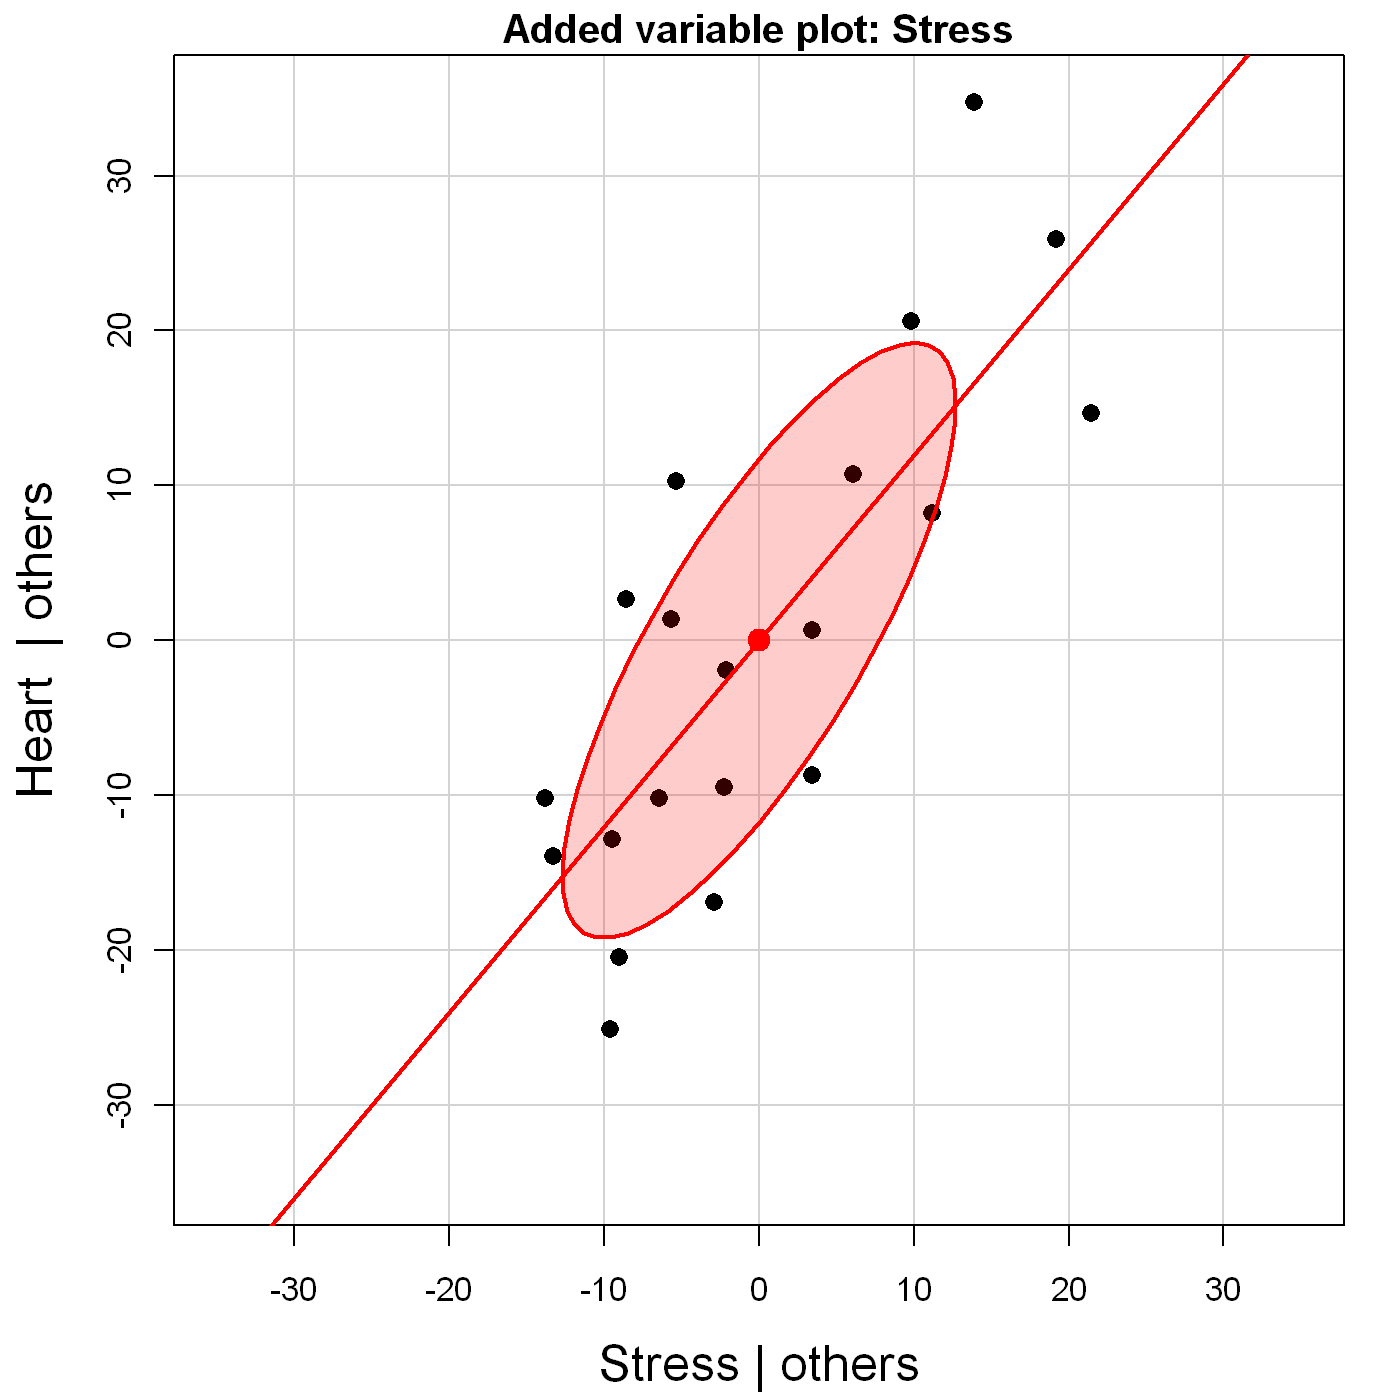
\includegraphics[width=1\linewidth]{fig/coffee-avplot1}
%  \caption{}%
%  \label{fig:}
 \end{minipage}%
 \hfill
 \begin{minipage}[b]{.49\linewidth}
  \centering
  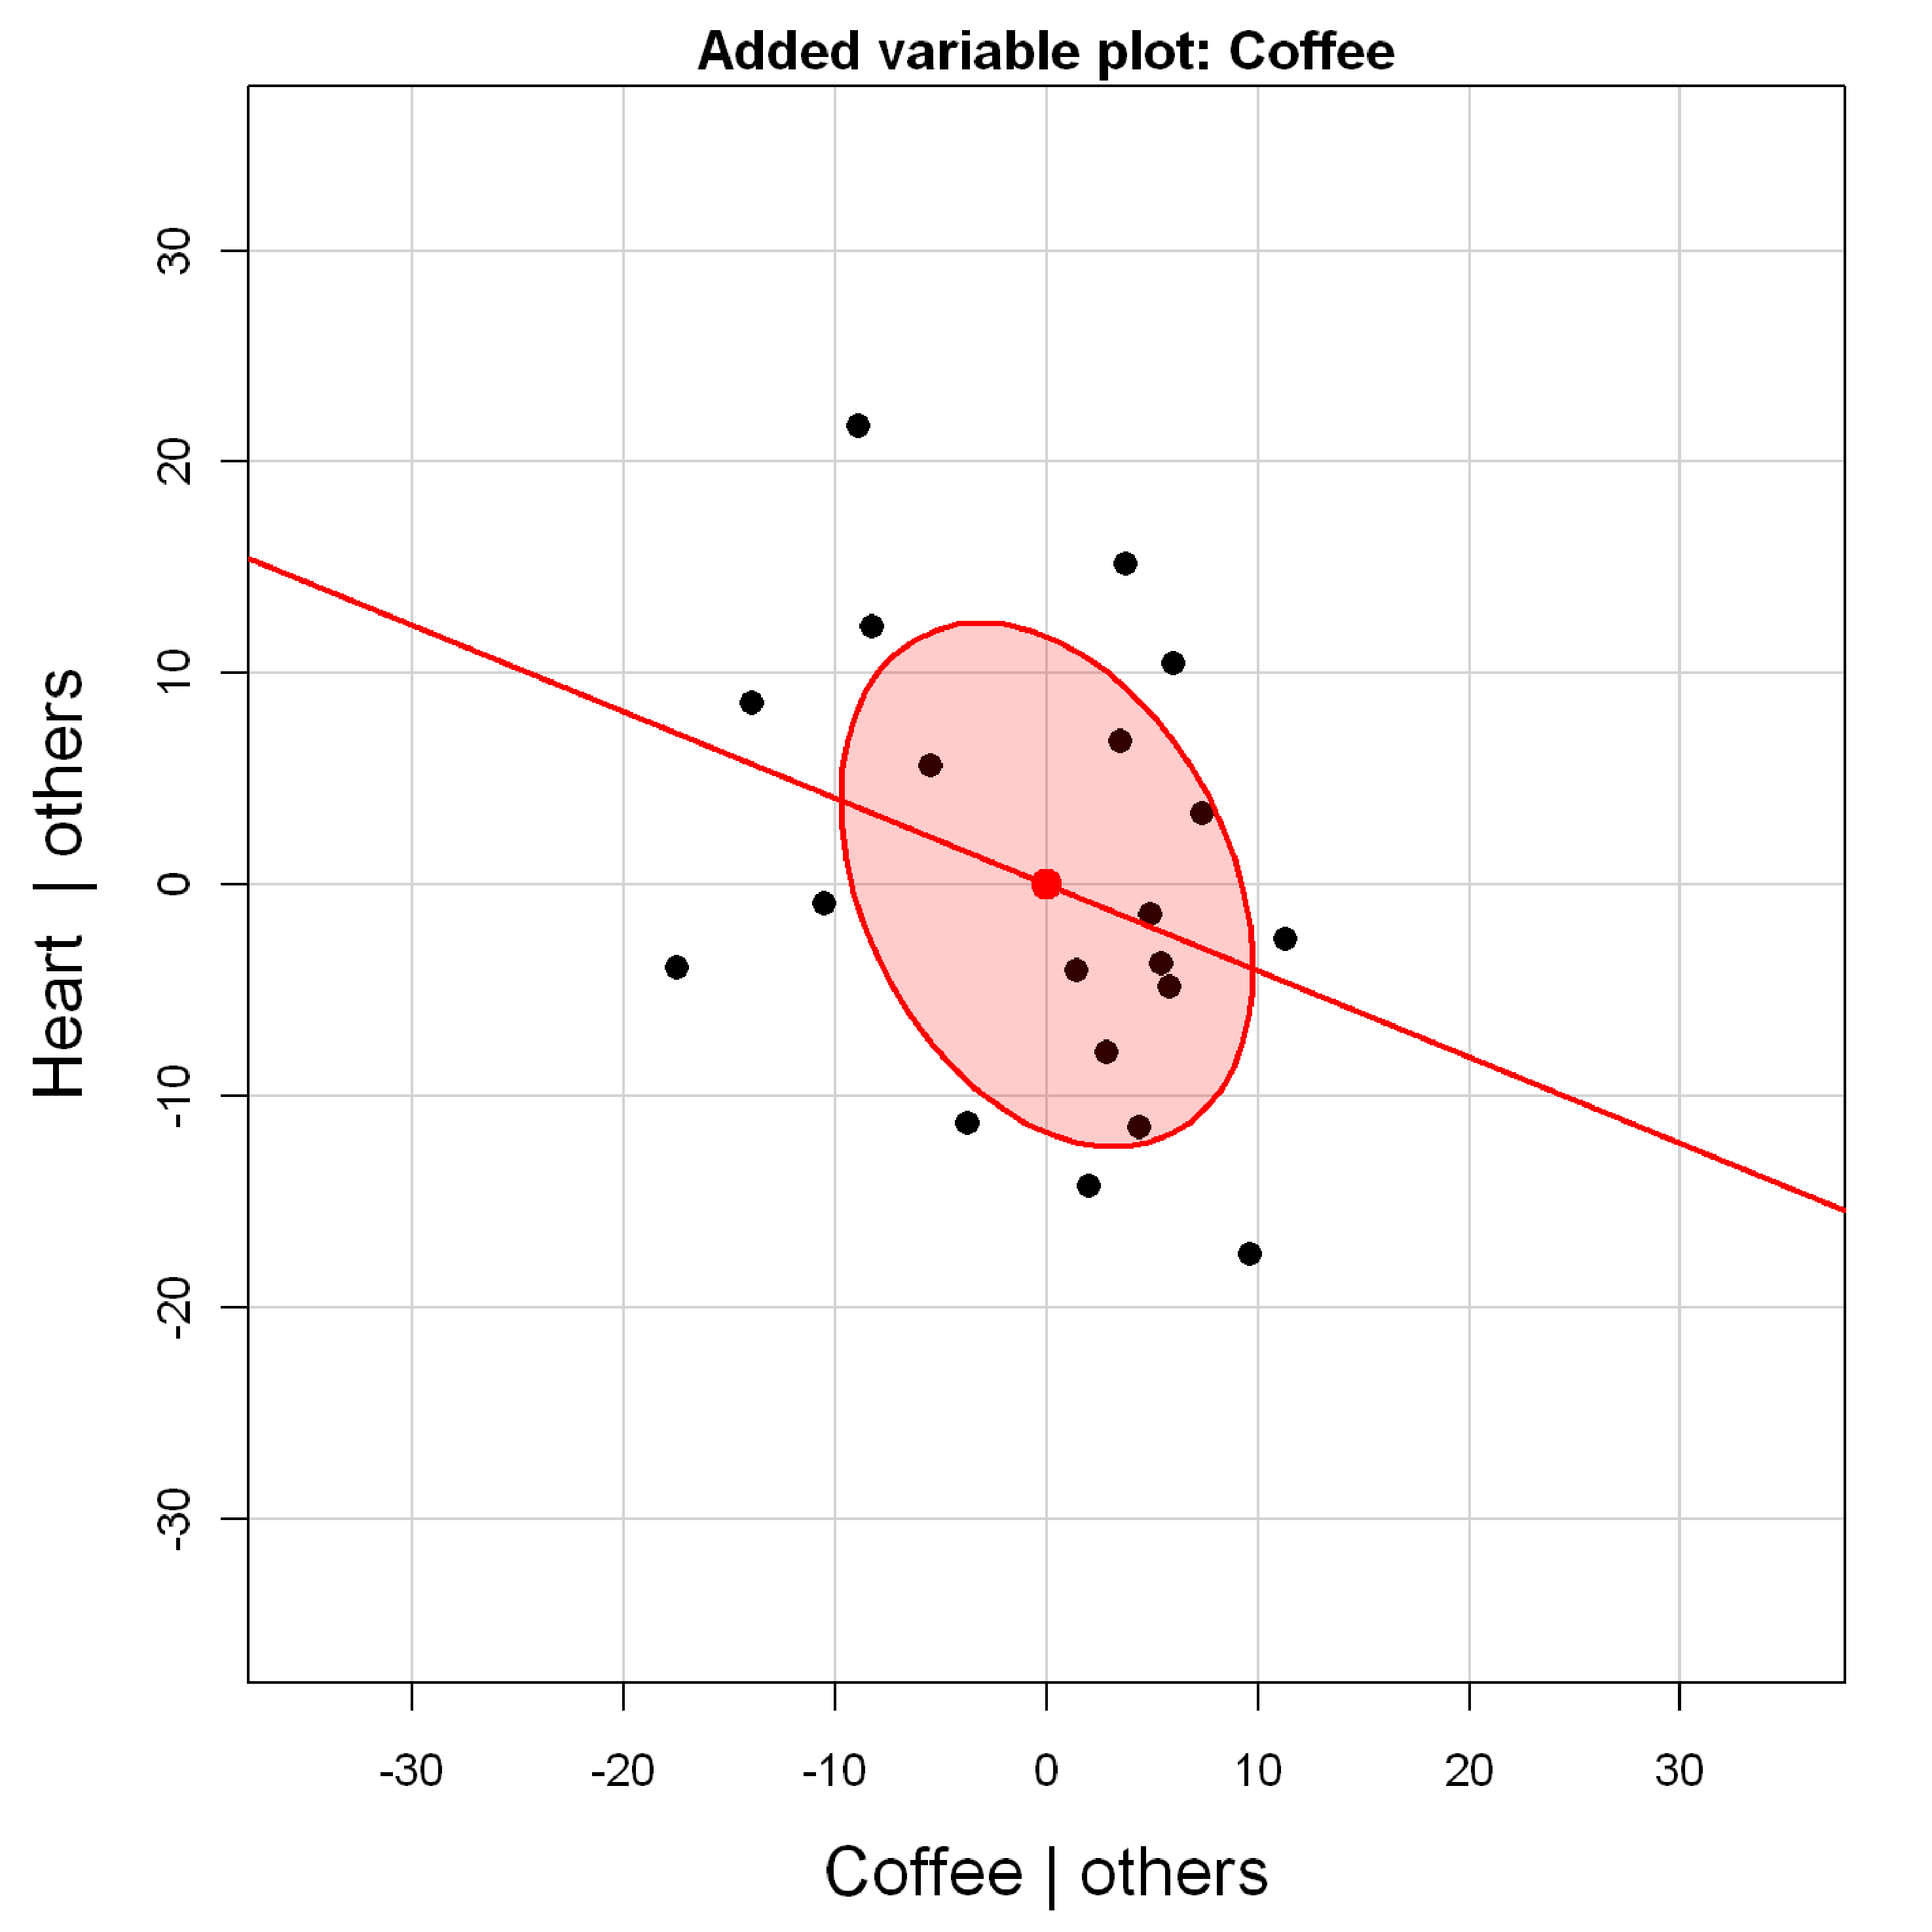
\includegraphics[width=1\linewidth]{fig/coffee-avplot2}
 \end{minipage}
  \caption{Added variable plots for Stress and Coffee in the multiple regression predicting Heart disease.
Each panel also shows the 50\% conditional data ellipse for partial residuals, $(\vec{x}_k^\star, \vec{y}^\star)$, shaded red. 
}
  \label{fig:coffee-avplot-A}
\end{figure}

Formally, we express the standard linear model in vector form as
$\widehat{\vec{y}} \equiv \widehat{\vec{y}} \given \mat{X} = \beta_0 \vec{1} + \beta_1 \vec{x}_1 + \beta_2 \vec{x}_2 + \dots +  \beta_p \vec{x}_p$
with model matrix $\mat{X} = [ \vec{1}, \vec{x}_1, \dots \vec{x}_p ]$.
Let $\mat{X}[-k]$ be the model matrix omitting the column for variable $k$. 
Then algebraically, the added variable plot for variable $k$ is the scatterplot of the residuals $(\vec{x}^\star_k, \vec{y}^\star)$ from
two auxillary regressions, fitting $\vec{y}$ and $\vec{x}_k$ from $\mat{X}[-k]$,
\begin{eqnarray*}
 \vec{y}^\star   & \equiv & \vec{y} \given \textrm{others}  =  \vec{y} - \widehat{\vec{y}} \given \mat{X}[-k] \\
 \vec{x}^\star_k & \equiv & \vec{x}_k \given \textrm{others}  =  \vec{x}_k - \widehat{\vec{x}}_k \given \mat{X}[-k]  \period \\
\end{eqnarray*}
(Computationally, these quantities can all be calculated \citep{VellemanWelsh:81} from the results of a single regression for the full model.)
 
Geometrically, in data space, the fitted vector $\widehat{\vec{y}}$ is the orthogonal projection of $\vec{y}$
onto the subspace spanned by $\mat{X}$. Then $\vec{y}^\star$ and $\vec{x}^\star_k$ are the projections onto
the orthogonal complement of the subspace spanned by $\mat{X}[-k]$, so
the simple regression of $\vec{y}^\star$ on $\vec{x}^\star_k$ has slope $\beta_k$ in the full model,
and the residuals from the line $\vec{y}^\star = \beta_k \vec{x}^\star_k$ in this plot are identically
the residuals from the overall regression of $\vec{y}$ on $\mat{X}$. 

Another way to describe this is that the added variable plot (AVP) for $x_k$ is a 2D projection of the space of
$(\vec{y}, \mat{X})$, viewed in the plane defined by the intersection of two hyperplanes:
the plane of the regression of $\vec{y}$ on all of $\mat{X}$, and the plane of regression of 
$\vec{y}$ on $\mat{X}[-k]$. A third plane, that of the regression of $x_k$ on $\mat{X}[-k]$
also intersects in this space, and defines the horizontal axis in the added variable plot.

%For three variables, $(y, x_1, x_2)$, the added variable plot for, say $x_1$, has particularly simple geometric interpretations in 3D in terms
%of the fitted planes for the full model, $y \sim x_1 + x_2$, the marginal model, $y \sim  x_2$

\figref{fig:coffee-avplot-A} shows added variable plots for Stress and Coffee in the multiple regression predicting Heart disease,
supplemented by data ellipses for the partial residuals $(\vec{x}_k^\star, \vec{y}^\star)$.  With reference to the properties
of data ellipses in marginal scatterplots (see \figref{fig:ellipses-demo}), the following visual properties (among others)
are useful in this discussion.  These follow simply from translating ``marginal'' into ``conditional'' (or ``partial'')
in the present context.

\begin{figure}[htb]
 \begin{minipage}[b]{.49\linewidth}
  \centering
  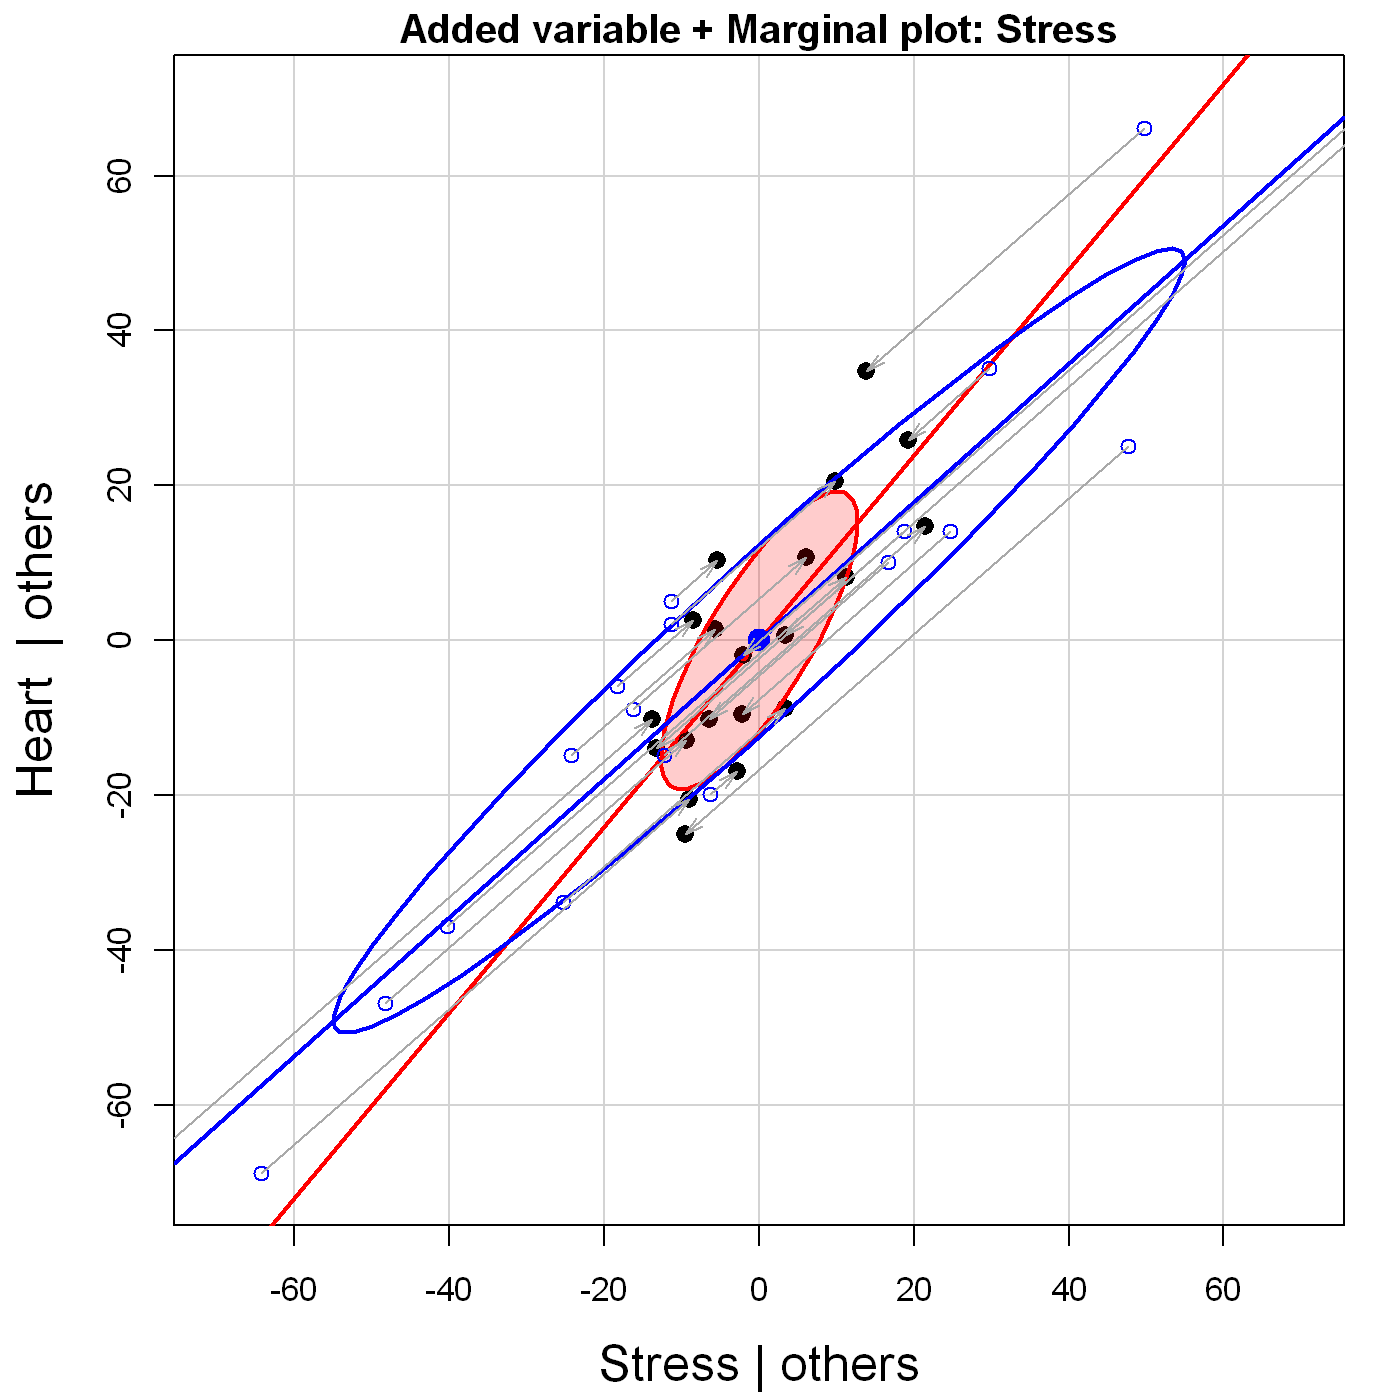
\includegraphics[width=1\linewidth]{fig/coffee-avplot3}
%  \caption{}%
%  \label{fig:}
 \end{minipage}%
 \hfill
 \begin{minipage}[b]{.49\linewidth}
  \centering
  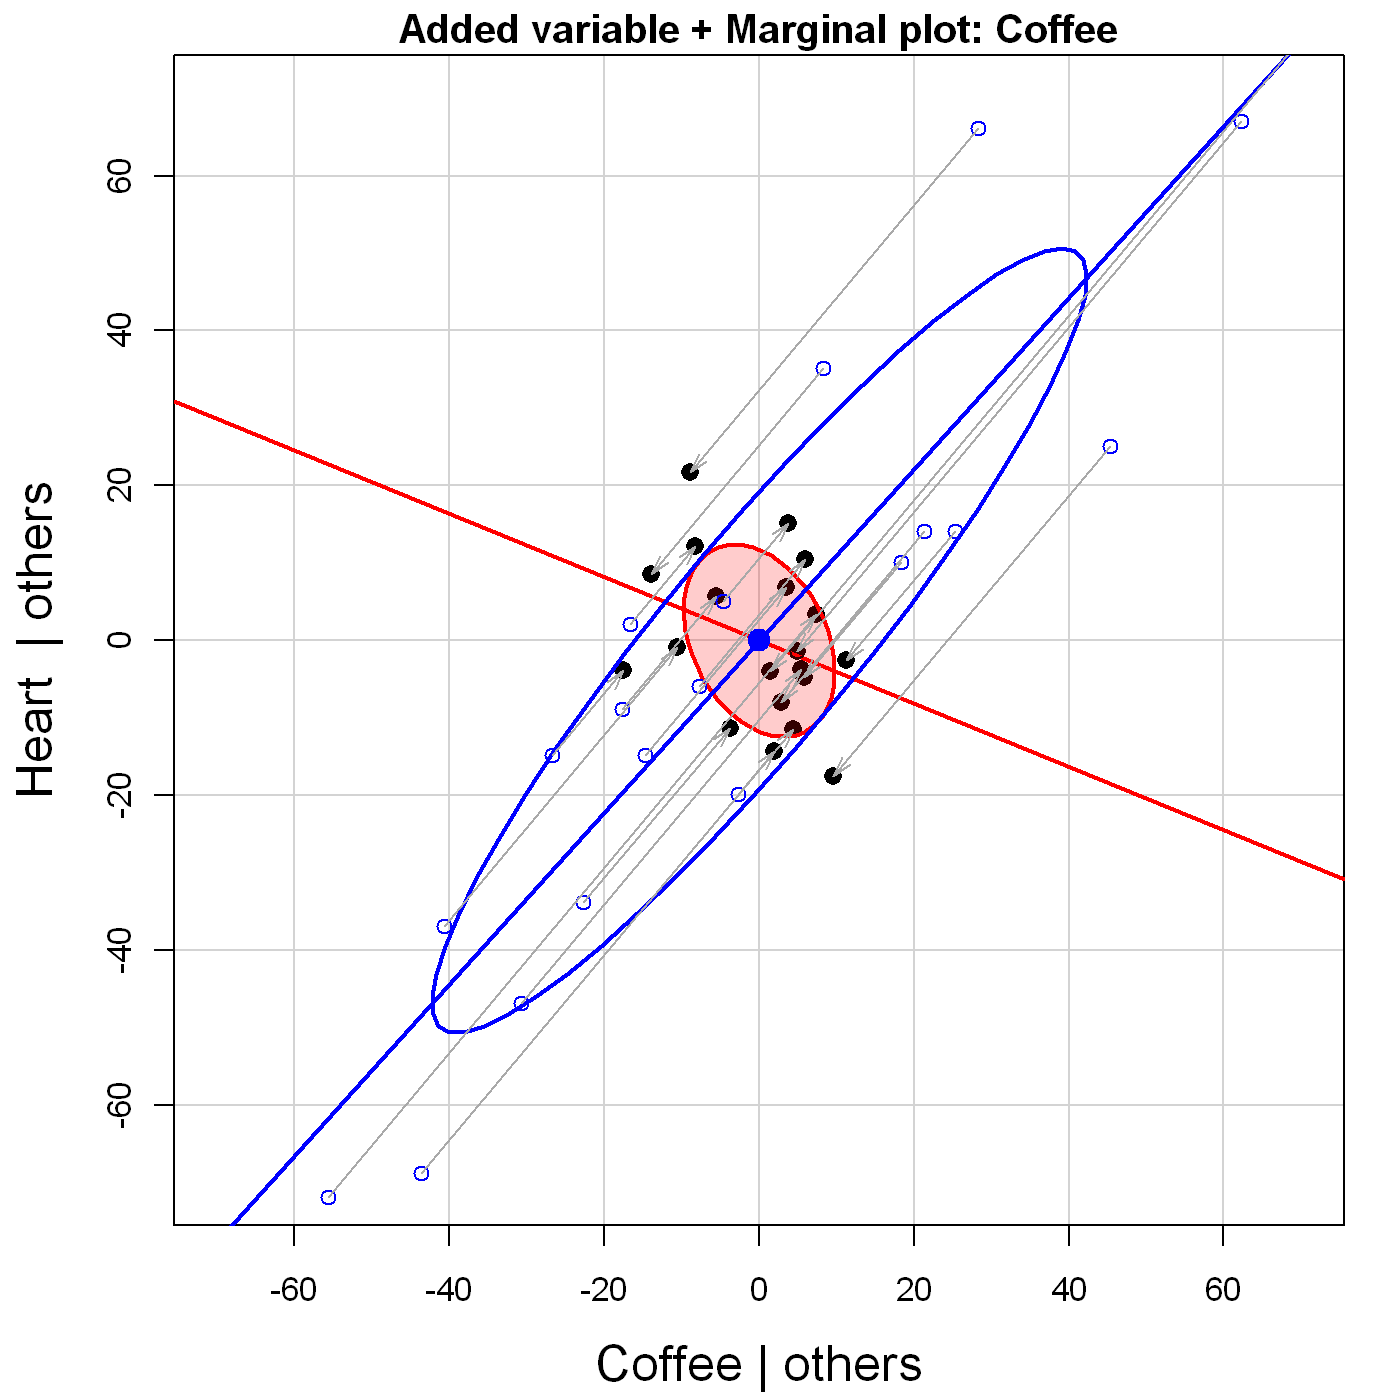
\includegraphics[width=1\linewidth]{fig/coffee-avplot4}
 \end{minipage}
  \caption{Added variable $+$ marginal plots for Stress and Coffee in the multiple regression predicting Heart disease.
Each panel shows the 50\% conditional data ellipse for partial residuals (shaded, red) as well as the marginal 50\% 
data ellipse for the $(x, y)$ variables, shifted to the origin.
Arrows connect the mean-centered marginal points (open circles) to the partial residual points (filled circles).}
  \label{fig:coffee-avplot-B}
\end{figure}

\begin{itemize*}
 \item the data ellipse of the AVP for $(x_k, y)$ is to the estimation of a coefficient in a multiple regression as
 the data ellipse of $(x, y)$ is to simple regression. Thus:
 \item the simple regression least squares fit of $\vec{y}^\star$ on $\vec{x}_k^\star$ has slope $\beta_k$,
 the partial slope for $x_k$ in the full model (and intercept = 0). 
 \item the correlation between $\vec{x}_k^\star$ and $\vec{y}^\star$ seen in the shape of the data ellipse
 is the partial correlation between $y$ and $x_k$ with all other predictors in $\mat{X}[-k]$ partialled out.
 \item the horizontal half-width of the data ellipse is proportional to the unique standard deviation of
 $x_k$, remaining after all other predictors have been accounted for.  This provides a visual interpretation
 of variance inflation, as we describe below.
 \item the vertical half-width of the data ellipse is proportional to the residual standard deviation of
 $y$, remaining after all other predictors have been accounted for.
 \item the squared horizontal positions, $(\vec{x}_k^\star)^2$, in the plot give the partial contributions
 to leverage for $x_k$, and the vertical positions, $\vec{y}^\star$, give the partial residuals.
 \item The last two points imply that the collection of added variable plots for $\vec{y}$ and
 $\mat{X}$ provide an easy way to visualize the influences that individual observations have on
 the esimation of \emph{each} coefficient in a given model.
\end{itemize*}


Elliptic insights also permits us to go further, to show the relation between conditional and marginal views
directly.
\figref{fig:coffee-avplot-B} shows the same added variable plots for Heart disease on Stress and Coffee
as in \figref{fig:coffee-avplot-A} (with a zoomed-out scaling), but here we also overlay the 
marginal data ellipses for $(x, y)$,
and and marginal regression lines for Stress and Coffee separately.  In 3D data space,
these are just the shadows (projections) of the data ellipsoid onto the planes defined by the
partial variables.  In 2D, AVP space, these are just the marginal data ellipses translated to
the origin.

The most obvious feature is that the AVP for Coffee has a negative slope in the conditional
plot (suggesting that controlling for Stress, coffee consumption is bad for your heart), while
in the marginal plot increasing coffee seems to be good for your heart. This serves as a
regression example of Simpson's paradox that we considered earlier.

Less obvious is the fact that 
the marginal and AVP ellipses are easily visualized as a shadow versus a slice of the full data ellipsoid. 
Thus, the AVP ellipse must be contained in the marginal ellipse, as we can see in \figref{fig:coffee-avplot-B}.
If there are only two $x$s, then the AVP ellipse must touch the marginal ellipse at some points. 
% This implies interesting contraints among the three quantities: improvement in fit, VIF and change from marginal to conditional slope.
The shrinkage of the intersection of the AVP ellipse with the $y$ axis represents improvement in fit due to other $x$s.

More importantly, the shrinkage of the width (projected onto a horizontal axis) represents the 
square root of the variance inflation factor (VIF), which can be shown to be the ratio of the horizontal
width of the marginal ellipse of $(x_k, y)$, with standard deviation $s(x_k)$ to the width of the conditional
ellipse of $(x_k^\star, y^\star)$, with standard deviation $s(x_k \given \textrm{others})$.
This geometry implies interesting contraints among the three quantities: improvement in fit, VIF and change from the marginal to conditional slope.

Finally, \figref{fig:coffee-avplot-B} also shows how conditioning on other predictors works for individual
observations, where each point for  $(\vec{x}_k^\star, \vec{y}^\star)$ is the image of $(\vec{x}_k, \vec{y})$ 
along the path of the marginal regression. This reminds us that the AVP is a 2D projection of the full space,
where the regression plane of $y$ on $\mat{X}[-k]$ becomes the vertical axis and 
the regression plane of $x_k$ on $\mat{X}[-k]$ becomes the horizontal axis.

